% https://tex.stackexchange.com/a/295109/173708

\documentclass[tikz,border=5]{standalone}
\begin{document} 
	
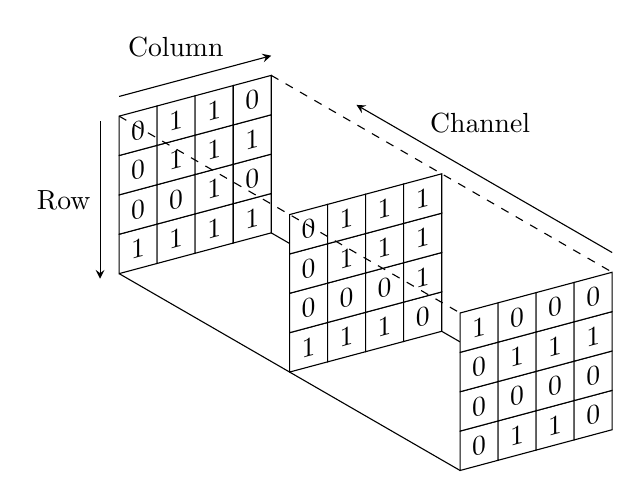
\begin{tikzpicture}[x=(15:.5cm), y=(90:.5cm), z=(330:.5cm), >=stealth]
	\draw (0, 0, 0) -- (0, 0, 10) (4, 0, 0) -- (4, 0, 10);
	\foreach \z in {0, 5, 10} \foreach \x in {0,...,3}
	  \foreach \y [evaluate={\b=random(0, 1);}] in {0,...,3}
	    \filldraw [fill=white] (\x, \y, \z) -- (\x+1, \y, \z) -- (\x+1, \y+1, \z) --
	      (\x, \y+1, \z) -- cycle (\x+.5, \y+.5, \z) node [yslant=tan(15)] {\b};
	\draw [dashed] (0, 4, 0) -- (0, 4, 10) (4, 4, 0) -- (4, 4, 10);
	\draw [->] (0, 4.5, 0)  -- (4, 4.5, 0)   node [near end, above left] {Column};
	\draw [->] (-.5, 4, 0)  -- (-.5, 0, 0)   node [midway, left] {Row};
	\draw [->] (4, 4.5, 10) -- (4, 4.5, 2.5) node [near end, above right] {Channel};
\end{tikzpicture}%
\end{document}